\section*{Занятия 2}
\begin{exercise}[1] Десять команд случайным образом (по жребию) разбиваются на две разные подгруппы. 
	
	$| \Omega | = C^5_{10} C^5_5$
	
	\begin{enumerate}
		\item [(a)] Выбрать место для 2 сильнейших команд: 2 \\ Выбрать 4 команда для подгруппы 1: $C^4_8$ \\ Выбрать 4 команда для подгруппы 2: $C^4_4$ \\ Ответ: $\frac{2 C^4_8 C^4_4}{C^5_{10} C^5_5} = \frac{5}{9}$
		\item [(б)] Выбрать подгруппу для 2 команда: $C^1_2$ \\ Выбрать больше 3 команда этой группы: $C^3_8$ \\ Ответ: $\frac{C^1_2 C^3_8}{C^5_{10} C^5_5} = \frac{4}{9}$
		\item [(в)] Выбрать больше 3 команда первой группы: $C^3_8$ \\ Выбрать 5 команд второй группы: $C^5_5$ \\ Ответ: $\frac{C^3_8 C^5_5}{C^5_{10} C^5_5} = \frac{2}{9}$
	\end{enumerate}
\end{exercise}

\begin{exercise}[2]
	\begin{enumerate}
		\item [(а)] $| \Omega | = C^3_{52}$ \\ Выбрать тройку $C^1_4$, семарку $C^1_4$, туз $C^1_4$ \\ Ответ: $\frac{C^1_4 C^1_4 C^1_4}{C^3_{52}} = \frac{16}{5525}$
		\item [(б)] $| \Omega | = A^3_{52}$ (так как мы выберем последовательные карты) \\ Для три любых карт существует только один заказ, поэтому нужно выбрать атрибут первой карты $C^1_4$, второй $C^1_4$, третьей $C^1_4$ \\ Ответ: $\frac{C^1_4 C^1_4 C^1_4}{A^3_{52}} = \frac{8}{16575}$
	\end{enumerate}
\end{exercise}

\begin{exercise}[3]
	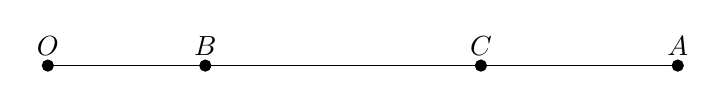
\begin{tikzpicture}
		\draw (-4,0) -- (4,0);
		\filldraw [black] (-4,0) circle (2pt) node[anchor=south]{$O$};
		\filldraw [black] (-2,0) circle (2pt) node[anchor=south]{$B$};
		\filldraw [black] (1.5,0) circle (2pt) node[anchor=south]{$C$};
		\filldraw [black] (4,0) circle (2pt) node[anchor=south]{$A$};
	\end{tikzpicture}
	
	Пусть $L$ - длина отрезка $OA$ \\ $x$ - длина отрезка $OB$ \\ $y$ - длина отрезка $BC$ \\ У нас есть: $\begin{cases}
		y < x \\ x +y < L \\ x > 0 \\ y > 0
	\end{cases}$
	
	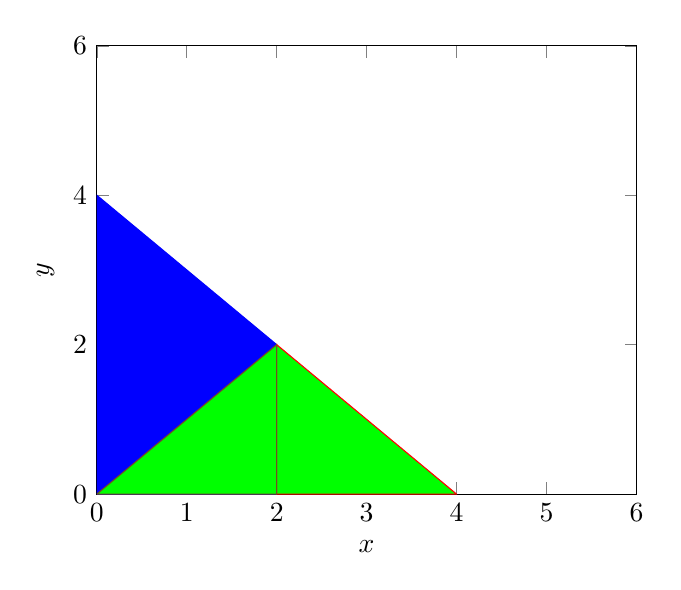
\begin{tikzpicture}
		\begin{axis}[
			xlabel=$x$, ylabel=$y$,
			xmin=0, ymin=0,
			xmax=6, ymax=6
			]
			\addplot+[mark=none, fill=blue, domain=0:2] {4-x} \closedcycle;
			\addplot+[mark=none, fill=green, domain=2:4] {4-x} \closedcycle;
			\addplot+[mark=none, domain=0:2, fill=green] {x} \closedcycle;
		\end{axis}
	\end{tikzpicture}
	
	Здесь, $| \Omega | = \frac{L^2}{2}$, а вероятность, которая удовлетворяет условии: $\frac{L \cdot \frac{L}{2}}{2} = \frac{L^2}{4}$ \\ Ответ: $\frac{L^2}{4} : \frac{L^2}{2} = \frac{1}{2}$
\end{exercise}

\begin{exercise}[4]
	$| \Omega | = 10!$ \\ Ответ: $\frac{1}{10!}$
\end{exercise}

\begin{exercise}[5]
	$| \Omega | = 8^4$
	\begin{enumerate}
		\item [(a)] Выбрать 4 этажа из 8: $A^4_8$ \\ Ответ: $\frac{A^4_8}{8^4} = \frac{105}{256}$
		\item [(б)] Этаж 6, 7, 8, 9, поэтому 4 этажа: $4^4$ \\ Ответ: $\frac{4^4}{8^4} = \frac{1}{16}$
		\item [(в)] 7 этажов: $7^4$ \\ Ответ: $\frac{7^4}{8^4} = \frac{2401}{4096}$
	\end{enumerate}
\end{exercise}

\begin{exercise}[6]
	$| \Omega | = 10^4=10000$
	\begin{enumerate}
		\item [(a)] Первое число имеет 9 вариантов (кроме 0). Другие числа имеют 10 вариантов \\ Ответ: $\frac{9 \cdot 10^3}{10^4} = 0,9$
		\item [(б)] Чтобы делится на 5, последнее число равно 0 или 5 \\ Ответ: $\frac{9 \cdot 10^2 \cdot 2}{10^4} = 0,18$
	\end{enumerate}
\end{exercise}

\begin{exercise}[7]
	$| \Omega | = C^{10}_{20}$ \\ Если билеты 1 и 2 не будет, тогда имеется 18 билетов, значит $C^{10}_{18}$ \\ Ответ: $\frac{C^{10}_{18}}{C^{10}_{20}} = \frac{9}{38}$
\end{exercise}

\begin{exercise}[8]
	$| \Omega | = C^4_{6+4+2} = C^4_{12}$ \\ Ответ: $\frac{C^4_{4+2}}{C^4_{12}} = \frac{1}{33}$
\end{exercise}

\begin{exercise}[9]
	$| \Omega | = 10!$ \\ 
	Рассмотрим 3 красного книги как 1, тогда у нас нес 8 книг. Найти места для 8 книг: $8!$ \\ 3 краного книга имеет $3!$ \\ Ответ: $\frac{8! 3!}{10!} = \frac{1}{15}$
\end{exercise}

\begin{exercise}[10]
	Каждая кость имеет 6 вариантов, поэтому $| \Omega | = 6^3$ \\ События А: кости выпадут разными гранями, то есть $6 \cdot 5 \cdot 4$ \\ Тогда, $P(A) = \frac{6 \cdot 5 \cdot 4}{6^3} = \frac{5}{9}$ \\ События B: на всех костях выпадет одинаковое число очков, то есть 6 чисел \\ Тогда $P(B) = \frac{6}{6^3} = \frac{1}{36}$
\end{exercise}

\begin{exercise}[11]
	У нас есть 5 пар ботинок, значит 10 ботинок. Поэтому $| \Omega | = C^2_{10}$ \\ Существуют 5 пар, то $P(A) = \frac{5}{C^2_{10}} = \frac{1}{9}$
\end{exercise}

\begin{exercise}[12]
	Тат как каждый участник может получит любый приз, поэтому $| \Omega | = 10^6$ \\ Данные 6 учасников получат по одному призу каждый, то $6!$ \\ Ответ: $\frac{6!}{10^6} = 0,00072$
\end{exercise}

\begin{exercise}[13]
	$| \Omega | = C^4_8 C^4_4$ \\ Выбрать 2 юношей и 2 девушек для группы 1: $C^2_4 C^2_4$ \\ Ответ: $\frac{C^2_4 C^2_4}{C^4_8 C^4_4} = \frac{18}{35}$
\end{exercise}

\begin{exercise}[14]
	\item [(a)] $P(A) = \frac{S_{\square}}{S_{\circ}} = \Big(\frac{2R}{\sqrt{2}}\Big)^2:(\pi R^2) = \frac{2}{\pi}$
	\item [(б)] $P(B) = \frac{S_{\triangle}}{S_{\circ}} = \Big[(R \sqrt{3})^2 \cdot \frac{\sqrt{3}}{4}\Big] : (\pi R^2) = \frac{3 \sqrt{3}}{4 \pi}$
\end{exercise}

\begin{exercise}[15] В течение суток к причалу независимо друг от друга
	
	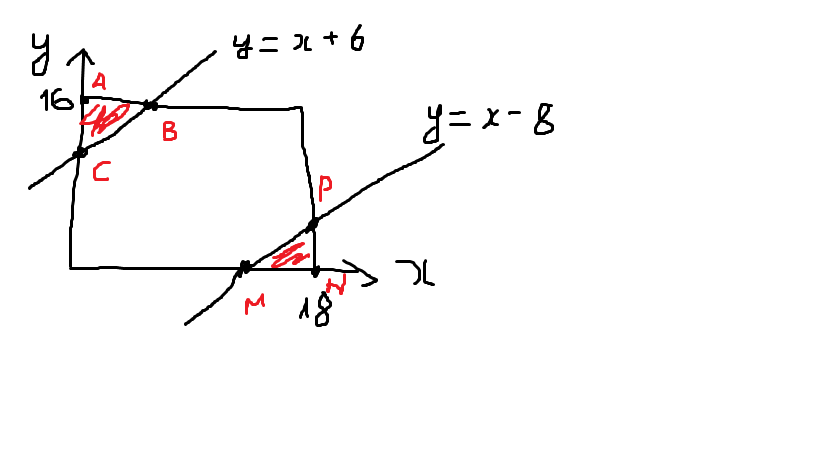
\includegraphics[scale=0.5]{exer15.png}
	
	Пусть $x$ - время первый сухогруз начинает разгрузиться и $y$ - время второй сухогруз начинает разгрузиться \\ Тогда, $x+6 \leq 24$ и $y+8 \leq 24 \Leftrightarrow x \leq 18$ и $y \leq 16$ \\ Cлучай 1: первый сухогруз начинает раньше чем второй, тогда $x+6 \leq y$ \\ Случай 2: второй сухогруз начинает раньше чем первый, тогда $y+8 \leq x$ \\ Получим $P(A) = \frac{S_{\triangle ABC} + S_{\triangle MNP}}{S_{\square}} = \Big(\frac{10 \cdot 10}{2} + \frac{10 \cdot 10}{2} \Big) : (16 \cdot 18) = \frac{25}{72}$ 
\end{exercise}